\documentclass[10pt]{article}
\usepackage[margin=1.5cm]{geometry}
\usepackage{graphicx,booktabs,amsmath,amssymb}
\usepackage[hidelinks]{hyperref}
\usepackage{fancyvrb,amsthm}
\usepackage{xr}
\externaldocument[M-]{../manuscript/main}
\newtheorem{propS}{Proposition}
\renewcommand{\thepropS}{S\arabic{propS}}
\newcommand{\PP}{\mathbb{P}}
\title{Supplementary Material for ``Innovation-Normalized Detection in Compound-Gaussian Clutter: Exact Laws, Conformal Thresholds and Certified Integration under Pulsed Interference''}
\author{M. U. Raza, S. Ahmed, and A. Ahmed}
\date{}
\begin{document}
\sloppy
\maketitle
\noindent All numbers below are generated from the saved outcomes in the project repository (\texttt{research/r7c}). Eleven protocols were frozen and hash-recorded before their outcomes were computed: the main IPIX study (\texttt{PROTOCOL.md}), single-pulse detection (\texttt{detection/PROTOCOL\_DETECTION.md}), onset (\texttt{detection/PROTOCOL\_ONSET.md}), baselines (\texttt{baselines/PROTOCOL\_BASELINES.md}), the 77~GHz radar (\texttt{jku/PROTOCOL\_JKU.md}), classical detectors, gradual emergence and ACI contamination (\texttt{r10/PROTOCOL\_R10.md}), order-statistic normalization with real interference (\texttt{r11/PROTOCOL\_R11.md}), low false-alarm calibration, ANMF baselines, the real IPIX target and certified integration under pulsed interference (\texttt{r12/PROTOCOL\_R12.md}), the guarded scale, clip level, certified trimming and pulse blanking (\texttt{r14/PROTOCOL\_R14.md}), the confirmation on NetRAD S-band sea clutter (\texttt{r15/PROTOCOL\_R15.md}), and real onsets of a walking person at 77~GHz (\texttt{r17/PROTOCOL\_R17.md}, frozen and pushed before the data were obtained). A further protocol (\texttt{sdrdsp/PROTOCOL\_SDRDSP.md}) was frozen before the SDRDSP data were obtained.

Study labels R7--R17 name these protocols in the repository (R1--R6 were development iterations on synthetic data); they are used only here. Deviations from the frozen protocols are listed in Section~\ref{sup:deviations}.

\section{Data exposure}
Table~\ref{tab:exposure} states which data each stage used, so that the strength of each validation claim can be judged. Only the hold-out series, the 77~GHz data and NetRAD were not used while the methods were being developed.
\begin{table}[h]
\centering\small
\caption{Data exposure by stage. ``Seen'' means that outcomes on these data were computed while methods, orders or comparisons could still change.}
\label{tab:exposure}
\begin{tabular}{p{4.3cm}p{5.2cm}p{6.2cm}}
\toprule
Data & Used for & Status of the reported results\\
\midrule
IPIX, 14 sessions, rotation 1 & Method development (R1--R7): method list, model orders, comparisons & Seen; not reported\\
IPIX, same sessions, rotations 2--3 & Main study, detection, onset, baselines, classical detectors, order-statistic scores (R7--R11) & Frozen-protocol evaluation, computed once per protocol; the recordings were seen in rotation 1, so this is not an untouched confirmation\\
IPIX, day transfer & Transfer and ACI analyses & Frozen-protocol evaluation on the same recordings\\
IPIX \#269, \#287 & Hold-out & Hashed and unopened until the main analysis was complete; evaluated once (small test sets)\\
JKU 77~GHz, reference run & Second-radar study & Not used in development; frozen protocol; the general-form gain curve is post hoc\\
JKU 77~GHz, interference runs A and C & Real-interference test (R11); certified integration (R12) & R11: only chirp-hit statistics inspected before its protocol. R12: R11 outcomes on these runs had been seen\\
IPIX, rotations 2--3 & Guarded scale, clip level, trimming, blanking (R14) & Frozen-protocol evaluation, computed once; same recordings as R7--R12\\
IPIX, primary target cells & Real-target study (R12) & Excluded from the R7--R11 clutter studies; a development check (V4, before R7) had run IN-ARCP on the primary cell and found it blind. Frozen protocol, evaluated once\\
NetRAD S-band, node 3, 14 recordings & Second-radar sea-clutter confirmation (R15) & Untouched: protocol frozen before any statistic of the samples was computed; evaluated once\\
JKU 77~GHz, pedestrian run (scenario A) & Real onsets of a walking person (R17) & Untouched: protocol frozen and pushed before the file was downloaded; evaluated once; descriptive (E1 not met)\\
SDRDSP (pending) & Further sea-clutter confirmation & Protocol frozen and hashed before the data were obtained\\
\bottomrule
\end{tabular}
\end{table}

\section{Protocol deviations}\label{sup:deviations}
\begin{itemize}
\item Main IPIX study: before any run, an encoding error in the protocol file was repaired byte-exactly and the hash rewritten; no outcome had been computed. A GPU backend was added for the likelihood evaluation of the noise-aware fit; it gives identical fitted parameters to the CPU path.
\item Second radar: the descriptive hit rule summed range bins 20--247 instead of 20--250, because the fixed preprocessing removes bins above 247. The general-form gain curve was chosen after the pre-specified matched form failed to capture the magnitude of the measured gain, so it is post hoc.
\item Order-statistic study (R11): the protocol's rationale counted $j+1$ target-corrupted history innovations at look $j$ after onset; the correct count, $j$, was adopted after the data were seen. The data follow the corrected count, and the main text uses only the corrected statement.
\item Final study (R12): before the real-data runs, the numerical search for the Fisher's $g$ threshold was re-bracketed; the law is unchanged.
\end{itemize}

\section{Unmet expectations}\label{sup:unmet}
Each expected value was written down before the outcome was computed. Of the 53 outcomes predicted for the last four studies, thirteen were not met and four, all from the pedestrian study, were left without a verdict.
\begin{itemize}
\item Pedestrian study (R17; E1 not met, E2--E5 without a verdict): the onsets were expected in at least eight distinct five-frame blocks and fell in seven, because the person was tracked for only about six seconds. Every other result is therefore descriptive; all lie on the side the protocol expected (Section~\ref{sup:r17}).
\item Final IPIX study (R12; 12 of 18 met): calibration of the saturating clipped statistic; the Tyler law (expected within twofold); the CA power detector's white-noise law (expected off more than threefold); the cost of clipping (expected at most 1.5~dB); false alarms of non-coherent integration under real FMCW interference (expected at least fivefold in both runs); and the gain of AR gap reconstruction (expected at least 1~dB).
\item Improvement study (R14; 12 of 15 met): the guard's onset cost, the certificate at $10^{-3}$ and the cost of trimming (Section~\ref{sup:r14}).
\item NetRAD confirmation (R15; 12 of 15 met): calibration of six statistics at $10^{-4}$, the pivotality ranking against CA16, and a rise of false alarms in segments with flagged pulses (Section~\ref{sup:r15}).
\item Main IPIX study ($m=16$, $\alpha=0.1$; radius relative to IN-ARCP): the noise-aware gain was expected to concentrate in noise-affected sessions. It did for NA-AR(1) (0.915 noisy against 0.989 clean) but not for NA-AR(2) and NA-AR(4) (0.871 and 0.866 noisy against 0.739 and 0.709 clean), whose gain comes mainly from the AR clutter dynamics (expectation Q1, mixed).
\item Onset study: the gain of IN-ARCP over the long-window power detector was expected to shrink below 3~dB by an 8-pulse dwell. It persisted: 8.4~dB [5.2, 11.1] at $P_{\rm d}=0.5$ (expectation O3, refuted).
\item 77~GHz radar: the noise-aware scores were expected to be flatter than IN-ARCP across CNR classes. The AR(4) version was (mean largest class deviation 0.055 against 0.066); the AR(1) version was not (0.067; expectation J2, mixed).
\item Classical detectors (R10). The R10 output below prints expectation R1 as FAILED. It is met in substance. For a target that rises over $L$ pulses, reaching full amplitude at the first look, IN-ARCP's first-look gain over the long-window power detector (CAloc in the paper) falls from 9.86 to 8.65 to 4.65~dB for $L=1,4,8$. At $L=16$, CAloc reaches $P_{\rm d}=0.5$ at 9.1~dB while IN-ARCP stays below it up to 25~dB, so the gain is below $-15.9$~dB, well under the 5~dB bound. PAMF-H was expected to need at least 3~dB less SCR than integrated IN-ARCP over an 8-pulse dwell at $P_{\rm d}=0.5$; it needed 1.0~dB [0.3, 1.7] less (4.0~dB at $P_{\rm d}=0.9$). Gated ACI was expected to keep the clean false-alarm rate within $[0.8,1.2]\alpha$ at 5\% target contamination; it gave $0.55\alpha$ ($\gamma=0.02$) and $0.68\alpha$ ($\gamma=0.005$).
\item Order-statistic study (R11; 2 of 11 met): quintile false-alarm spread of the median OS score at most 2.0 (2.06); its cost for abrupt targets at most 1.5~dB (1.99~dB [0.89, 3.39]; Corollary~3 gives 0.69~dB); a first-look gain of at least 3~dB over IN-ARCP for 8-pulse ramps (1.46~dB); the integrated OS score closing half of integrated IN-ARCP's gap to PAMF-H at $P_{\rm d}=0.9$ (it was 2.5~dB worse); OS-law coverage error at most 0.015 (0.021); on the dense real-interference run, the OS score halving IN-ARCP's masking (drops 0.39 and 0.35), zeroing cutting the hit-pulse false-alarm rate by half (39\%), and the OS score after zeroing within 0.5~dB of IN-ARCP (0.71~dB worse); on the reference run, IN-ARCP beating CA16 (CA16 was 0.78~dB better, the loss Proposition~2 predicts for $c<1$).
\end{itemize}

\section{Hold-out series}
Two further McMaster series (\#269 and \#287, the widely used ``high'' and ``low'' sea-state files, one provider-preprocessed VV cell each, from the same 1993 campaign) were hashed and left unopened until the main analysis was complete, and then evaluated once (Table~\ref{tab:holdout}). They confirm the direction of the main result, with larger gains. They also show a case in which the classical Gaussian threshold over-covers while conformal IN-ARCP stays near nominal. Their test sets are small (about 165 episodes per unit), so the hold-out is a directional check. Mondrian calibration returns infinite regions at $1-\alpha=0.99$ there, because each bin receives fewer calibration episodes than the rank requires.
\begin{table}[h]
\centering\small
\caption{Hold-out series \#269 and \#287 ($1-\alpha=0.90$; six units per column).}
\label{tab:holdout}
\begin{tabular}{lcccc}
\toprule
 & \multicolumn{2}{c}{$m=8$} & \multicolumn{2}{c}{$m=16$}\\
\cmidrule(lr){2-3}\cmidrule(lr){4-5}
Method & Radius ratio & Coverage (min) & Radius ratio & Coverage (min)\\
\midrule
Noise-aware AR(4) (proposed) & 0.454 & 0.890 (0.816) & 0.498 & 0.893 (0.847)\\
Noise-aware AR(2) (proposed) & 0.541 & 0.887 (0.828) & 0.533 & 0.895 (0.859)\\
AR(4), innovation-normalized & 0.546 & 0.908 (0.847) & 0.515 & 0.906 (0.883)\\
AR(2), innovation-normalized & 0.582 & 0.905 (0.840) & 0.572 & 0.906 (0.871)\\
Noise-aware AR(1) & 0.921 & 0.898 (0.840) & 0.921 & 0.903 (0.859)\\
IN-ARCP, AR(1) & 1.000 & 0.906 (0.853) & 1.000 & 0.910 (0.859)\\
Gaussian plug-in of IN-ARCP & 1.178 & 0.949 (0.896) & 1.104 & 0.945 (0.895)\\
Mondrian IN-ARCP & 1.000 & 0.895 (0.804) & 0.981 & 0.896 (0.810)\\
Learned-scale CP & 0.629 & 0.893 (0.804) & 0.662 & 0.919 (0.791)\\
Invariant MLP CP & 1.809 & 0.884 (0.736) & 2.158 & 0.903 (0.761)\\
Raw-RMS normalized CP & 1.321 & 0.880 (0.706) & 1.243 & 0.887 (0.706)\\
Unnormalized CP & 1.142 & 0.868 (0.607) & 1.161 & 0.859 (0.589)\\
Gaussian plug-in of noise-aware AR(4) & 0.411 & 0.866 (0.816) & 0.472 & 0.856 (0.755)\\
\bottomrule
\end{tabular}

\end{table}

\section{Summary of the laws}\label{sup:laws}
Table~\ref{sup:tablaws} collects the laws of Section~\ref{M-sec:laws} of the paper and marks the results that are new.

\begin{table}[!t]
\centering\footnotesize
\caption{Laws of whitened-innovation detection, with the equation numbers of the paper (AR(1) speckle, true coefficient, compound-Gaussian clutter; $S_w=S/(1-|\rho|^2)$, $w(\omega)=P/S_c(\omega)$, $\psi$ the P-ANMF threshold). New results are marked $^\ast$.}
\label{sup:tablaws}
\setlength{\tabcolsep}{3pt}
\begin{tabular}{lll}
\toprule
Detector & $P_{\rm fa}$ & $P_{\rm d}$ (Swerling 1)\\
\midrule
Look at onset & $(1+q^2/m)^{-m}$ & $\big(1+\frac{q^2}{m(1+S_w)}\big)^{-m}$\\
Look $\ell$ after onset$^\ast$ & same & \eqref{M-eq:rank1}; horizon \eqref{M-eq:horizon}\\
Guard of $\Delta$ pulses & same & \eqref{M-eq:rank1} at $\ell-\Delta$\\
OS scale, onset & $\prod_{i<k}\frac{m-i}{m-i+q^2}$ & same at $\frac{q^2}{1+S_w}$\\
OS scale, after onset$^\ast$ & same & \eqref{M-eq:osstrong}; exact by quadrature\\
$K$-pulse integration & \eqref{M-eq:dwellpfa} & \eqref{M-eq:dwellpd}\\
P-ANMF, known $\omega$ & $(1-\psi)^{N-1}$ & \eqref{M-eq:panmf}: SCR $\times N w(\omega)$\\
P-ANMF, max over bins & Fisher's $g$ & inclusion--exclusion\\
Certified clip/binary$^\ast$ & $\le\alpha$, any amplitude & by calibration\\
Conformal threshold & Beta$(n{+}1{-}k_\alpha,k_\alpha)$ & Beta moment\\
\bottomrule
\end{tabular}
\end{table}

\section{Synthetic verification}
\begin{figure}[h]
\centering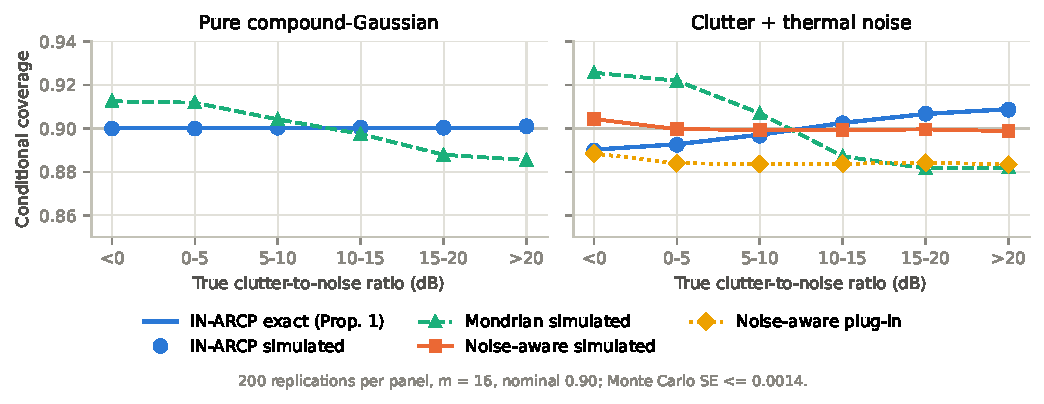
\includegraphics[width=.85\textwidth]{fig_synthetic_exact.pdf}
\caption{Synthetic verification: coverage conditional on the true clutter-to-noise ratio. The line is the exact law of Proposition~1; markers are simulation.}
\end{figure}

\section{Proof of Proposition 2 and the latent-texture Mondrian result}
Equation, proposition and theorem numbers without the prefix S refer to the paper.

\emph{Proposition~2.} If $e\sim\mathcal{CN}(0,v)$ and a Swerling-1 target of power $SP$ is added, a threshold test on $|e|^2/v$ at false-alarm probability $\alpha$ detects with probability $\alpha^{1/(1+SP/v)}$, while the power-only test on $|Y|^2/P$ detects with $\alpha^{1/(1+S)}$; equal $P_{\rm d}$ therefore requires SCRs in the ratio $G=P/v$. For the center $rH_m$ under \eqref{M-eq:r7model} with AR(1) speckle, $v=\nu\{c(1+|r|^2-2\Re\,\bar r\rho)+1+|r|^2\}$, which gives $G_{\rm IN}$. For the optimal predictor from the infinite past, $v$ is the one-step prediction-error variance of the AR(1)-plus-white-noise process, $\exp\{\int\log f\}$ by the Kolmogorov--Szeg\H{o} formula (Brockwell and Davis, \emph{Time Series: Theory and Methods}, 1991). With $f(\omega)=\nu\{c(1-|\rho|^2)+|1-\rho e^{-j\omega}|^2\}/|1-\rho e^{-j\omega}|^2$, the denominator contributes zero, and the numerator factorizes as $\nu V|1-\zeta e^{-j\omega}|^2$ with $V(1+|\zeta|^2)=\xi$, $V\zeta=\rho$ and $|\zeta|<1$, which gives $v=\nu V$ and $G_{\rm opt}$. Because the optimal predictor's error variance is at most that of any linear predictor, including $0$ and $rH_m$, $G_{\rm opt}\ge\max\{1,G_{\rm IN}\}$.

\emph{Latent-texture Mondrian calibration.} Mondrian (group-conditional) conformal prediction calibrates separately within bins of an observed statistic and is valid conditional on the observed bin; Dewolf et al.\ report that estimated taxonomies mix up the true classes. For a latent texture the consequence can be stated exactly.
\begin{propS}\label{prop:mondrian}
Let $\nu=0$ and $X=\sigma Z$, with $\sigma>0$ distributed as $G$, non-degenerate and independent of $Z\sim\mathcal{CN}(0,R)$. Let $S(Z)$ be a scale-invariant score with a continuous distribution function $F_S$ that is strictly increasing on its support, let $T(H)>0$ be continuous and homogeneous of degree one, and calibrate within fixed bins $B_b=[e_{b-1},e_b)$, $0=e_0<\dots<e_K=\infty$, $K\ge2$, of $T(H)$ with population quantiles $q_b$. Let $\mathcal C(\sigma)$ be the coverage conditional on the texture.
(i) If $S(Z)$ is independent of $T(Z_H)$, then $\mathcal C(\sigma)\equiv1-\alpha$.
(ii) If $S(Z)$ given $T(Z_H)=t$ is strictly stochastically decreasing in $t$, then $\lim_{\sigma\to\infty}\mathcal C(\sigma)=F_S(q_K)<1-\alpha<F_S(q_1)=\lim_{\sigma\to0}\mathcal C(\sigma)$, whereas the unbinned threshold gives a constant $\mathcal C(\sigma)$. Condition (ii) holds exactly for IN-ARCP at the true coefficient with $T=s_\rho$.
\end{propS}
\emph{Proof.}
Write $t=T(Z_H)$, so that the observed statistic is $T(X_H)=\sigma t$ and $S(X)=S(Z)$. For bin $b$ let $w_b(t)=\mathbb{P}\{\sigma t\in B_b\}$. Since $\sigma$ is independent of $Z$, for every $x$
\begin{equation}
\mathbb{P}\{S\le x,\ \sigma t\in B_b\}=\mathbb E\big[\varphi_x(t)\,w_b(t)\big],
\tag{S1}
\end{equation}
where $\varphi_x(t)=\mathbb{P}\{S\le x\mid t\}$.
(i) If $S$ is independent of $t$, then $\varphi_x\equiv F_S(x)$, every bin-conditional law of $S$ equals $F_S$, all $q_b$ equal $F_S^{-1}(1-\alpha)$ and $\mathcal C(\sigma)=1-\alpha$.

(ii) Let $x_0=F_S^{-1}(1-\alpha)$. For the top bin, $w_K(t)=\mathbb{P}\{\sigma\ge e_{K-1}/t\}$ is nondecreasing in $t$. Because $T$ is continuous, positive and homogeneous and $Z_H$ has full support, $t$ has full support on $(0,\infty)$; as $e_{K-1}/t$ then ranges over $(0,\infty)$ and $G$ is non-degenerate, $w_K(t)$ is not almost surely constant. By assumption $\varphi_{x_0}$ is strictly increasing. Let $t'$ be an independent copy of $t$, $D_\varphi=\varphi_{x_0}(t)-\varphi_{x_0}(t')$ and $\Delta_w=w_K(t)-w_K(t')$. Then
\[
\operatorname{Cov}\{\varphi_{x_0}(t),w_K(t)\}=\tfrac12\,\mathbb E[D_\varphi\Delta_w]>0,
\]
because $D_\varphi\Delta_w\ge0$, with strict inequality on the event $\{w_K(t)\ne w_K(t')\}$, which has positive probability. By (S1),
$\mathbb{P}\{S\le x_0\mid\sigma t\in B_K\}=\mathbb E[\varphi_{x_0}w_K]/\mathbb E[w_K]>\mathbb E[\varphi_{x_0}]=1-\alpha$.
The bin-conditional distribution function of $S$ is continuous, so there is $x_1<x_0$ at which it still exceeds $1-\alpha$; hence $q_K\le x_1<x_0$ and, $F_S$ being strictly increasing, $F_S(q_K)<1-\alpha$. For the bottom bin, $w_1(t)=\mathbb{P}\{\sigma<e_1/t\}$ is nonincreasing, the covariance is negative, and the same steps give $q_1>x_0$ and $F_S(q_1)>1-\alpha$.

The coverage at texture $\sigma$ is $\mathcal C(\sigma)=\sum_b\mathbb{P}\{S\le q_b,\ \sigma t\in B_b\}$. As $\sigma\to\infty$, $\sigma t\to\infty$ almost surely, so $\mathbf 1\{\sigma t\in B_K\}\to1$ and, by dominated convergence, $\mathcal C(\sigma)\to F_S(q_K)$; as $\sigma\to0$, $\mathcal C(\sigma)\to F_S(q_1)$. An unbinned threshold $q$ gives $\mathcal C(\sigma)=F_S(q)$ for every $\sigma$.

Finally, for IN-ARCP at $r=\rho$ and $T=s_\rho$, $S=|E|/t$ with the innovation $E$ independent of $Z_H$, so $\varphi_x(t)=\mathbb{P}\{|E|\le xt\}$ is strictly increasing in $t$, which is condition (ii). \hfill$\blacksquare$

\section{Zero-noise limit of the noise-aware score}
\begin{propS}\label{prop:reduce}
Let $R$ be AR(1) with coefficient $\rho$ and fix a nonzero history $h$. As $\nu\downarrow0$, $\nu\widehat c(h)\to h^{\mathsf H}R_H^{-1}h/m$, $\mu(h)\to\rho h_m$ and $s(h)\to s_\rho(h)$, so the NA score converges to the IN-ARCP score at $r=\rho$.
\end{propS}
\emph{Proof sketch.}
With $\gamma=\nu c$ the history log-likelihood converges locally uniformly on $\gamma>0$ to $-m\log\gamma-\gamma^{-1}h^{\mathsf H}R_H^{-1}h$, whose unique maximizer is $h^{\mathsf H}R_H^{-1}h/m$; coercivity at $0$ and $\infty$ gives convergence of the maximizers. The Markov property gives $\mu\to\rho h_m$, and $(1-|\rho|^2)R_H^{-1}=W_\rho^{\mathsf H}W_\rho$, with $W_\rho$ the bidiagonal whitening matrix, identifies the limiting predictive variance with $s_\rho(h)^2$.

\section{Texture-conditional coverage and disc widths on IPIX}
\begin{figure}[h]
\centering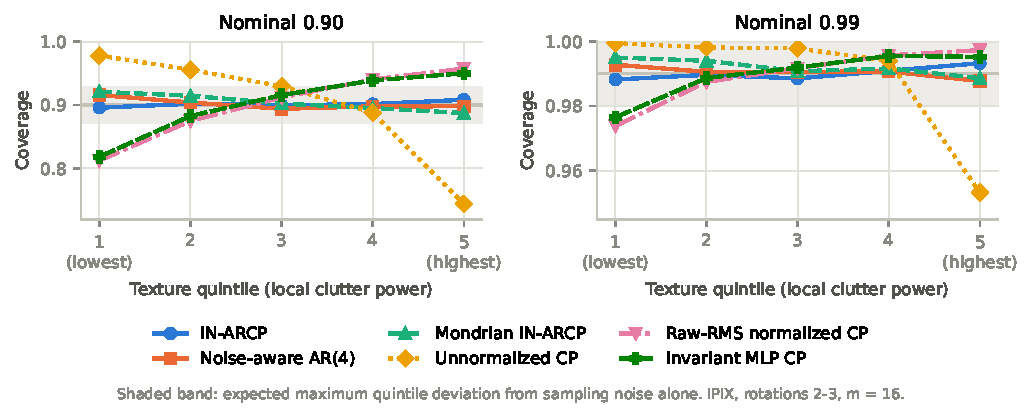
\includegraphics[width=.95\textwidth]{fig_texture_conditional.pdf}
\caption{Coverage by texture quintile on IPIX (rotations 2--3, $m=16$). Texture is proxied by the local clutter power ($\pm1024$ pulses, excluding the episode).}
\end{figure}
\begin{table}[h]
\centering\small
\caption{IPIX width and coverage ($m=16$; rotations 2--3; 56 units). Radius ratio: geometric mean over units of mean disc radius relative to IN-ARCP on the same test episodes, with 95\% day-cluster bootstrap interval. Max.\ dev.: mean over units of the largest absolute texture-quintile coverage deviation from nominal. At equal model order, NA-AR(4) has 0.891 [0.872, 0.905] times the radius of the innovation-normalized AR(4) disc.}
\resizebox{\textwidth}{!}{\begin{tabular}{lcccccc}
\toprule
 & \multicolumn{3}{c}{$1-\alpha=0.90$} & \multicolumn{3}{c}{$1-\alpha=0.99$}\\
\cmidrule(lr){2-4}\cmidrule(lr){5-7}
Method & Radius ratio [95\% CI] & Coverage & Max.\ dev. & Radius ratio [95\% CI] & Coverage & Max.\ dev.\\
\midrule
Noise-aware AR(4) (proposed) & 0.753 [0.714, 0.815] & 0.902 & 0.043 & 0.743 [0.706, 0.798] & 0.991 & 0.011\\
Noise-aware AR(2) (proposed) & 0.777 [0.748, 0.824] & 0.901 & 0.044 & 0.769 [0.745, 0.806] & 0.991 & 0.011\\
AR(4), innovation-normalized & 0.845 [0.805, 0.905] & 0.901 & 0.032 & 0.861 [0.822, 0.918] & 0.990 & 0.011\\
AR(2), innovation-normalized & 0.895 [0.855, 0.953] & 0.901 & 0.034 & 0.898 [0.857, 0.953] & 0.990 & 0.010\\
Noise-aware AR(1) & 0.966 [0.930, 0.994] & 0.901 & 0.042 & 0.952 [0.907, 0.989] & 0.990 & 0.011\\
IN-ARCP, AR(1) & 1 & 0.901 & 0.036 & 1 & 0.990 & 0.011\\
Gaussian plug-in of IN-ARCP & 0.995 [0.988, 1.002] & 0.900 & 0.034 & 0.993 [0.979, 1.005] & 0.990 & 0.011\\
Mondrian IN-ARCP & 0.980 [0.975, 0.984] & 0.904 & 0.043 & 0.998 [0.988, 1.006] & 0.992 & 0.011\\
Learned-scale CP & 0.921 [0.875, 0.990] & 0.900 & 0.039 & 1.072 [1.019, 1.147] & 0.991 & 0.012\\
Invariant MLP CP & 1.337 [1.288, 1.439] & 0.901 & 0.096 & 1.585 [1.489, 1.780] & 0.990 & 0.019\\
Raw-RMS normalized CP & 1.368 [1.320, 1.449] & 0.899 & 0.103 & 1.609 [1.533, 1.782] & 0.989 & 0.021\\
Unnormalized CP & 1.048 [1.010, 1.085] & 0.899 & 0.165 & 1.475 [1.261, 1.720] & 0.989 & 0.039\\
Gaussian plug-in of noise-aware AR(4) & 0.726 [0.687, 0.787] & 0.885 & 0.049 & 0.698 [0.659, 0.758] & 0.985 & 0.016\\
\midrule
Sampling-noise reference for max.\ dev. & & & 0.029 & & & 0.009\\
\bottomrule
\end{tabular}
}
\end{table}

\section{Day transfer and texture-proxy sensitivity}
\begin{table}[h]
\centering\small
\caption{Day transfer ($m=16$, $1-\alpha=0.90$): fit and calibrate on other days, test on each of six held-out days.}
\begin{tabular}{lccc}
\toprule
Method & Mean coverage & Worst held-out day & Radius ratio\\
\midrule
Noise-aware AR(4) (proposed) & 0.898 & 0.863 & 0.936\\
Noise-aware AR(2) (proposed) & 0.898 & 0.883 & 0.956\\
AR(4), innovation-normalized & 0.901 & 0.894 & 0.993\\
AR(2), innovation-normalized & 0.899 & 0.891 & 1.024\\
Noise-aware AR(1) & 0.900 & 0.882 & 1.037\\
IN-ARCP, AR(1) & 0.903 & 0.882 & 1.000\\
Gaussian plug-in of IN-ARCP & 0.906 & 0.893 & 1.006\\
Mondrian IN-ARCP & 0.907 & 0.881 & 0.984\\
Learned-scale CP & 0.898 & 0.774 & 0.967\\
Invariant MLP CP & 0.880 & 0.622 & 1.200\\
Raw-RMS normalized CP & 0.906 & 0.681 & 1.466\\
Unnormalized CP & 0.909 & 0.716 & 1.470\\
Gaussian plug-in of noise-aware AR(4) & 0.876 & 0.842 & 0.893\\
\bottomrule
\end{tabular}

\end{table}
\noindent Texture-proxy sensitivity (pre-specified windows; mean maximum quintile deviation at $1-\alpha=0.90$, $m=16$): with $\pm512$ pulses IN-ARCP 0.035, NA-AR(4) 0.043, unnormalized 0.181, neural center 0.103; with $\pm2048$ pulses IN-ARCP 0.033, unnormalized 0.141. The ranking is the same as with $\pm1024$.

\section{Additional figures for the IPIX study}
\begin{figure}[h]
\centering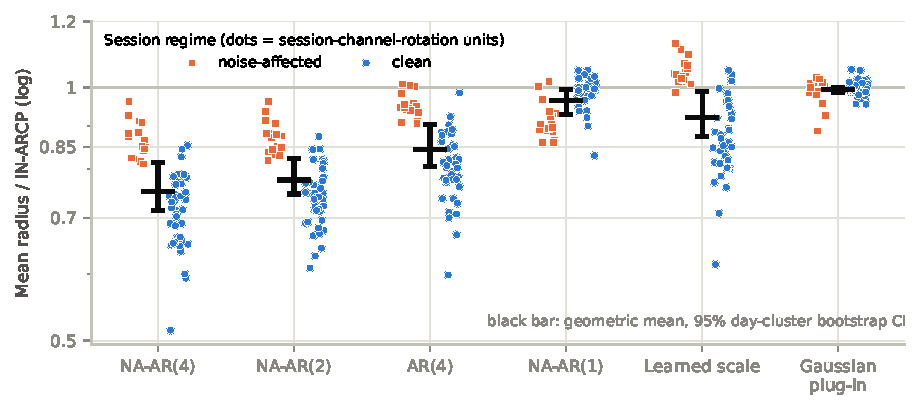
\includegraphics[width=.8\textwidth]{fig_width_ratios.pdf}
\caption{Per-unit radius relative to IN-ARCP at $1-\alpha=0.90$, $m=16$, by session regime (noise-affected: fitted noise power above 1\% of mean power).}
\end{figure}
\begin{figure}[h]
\centering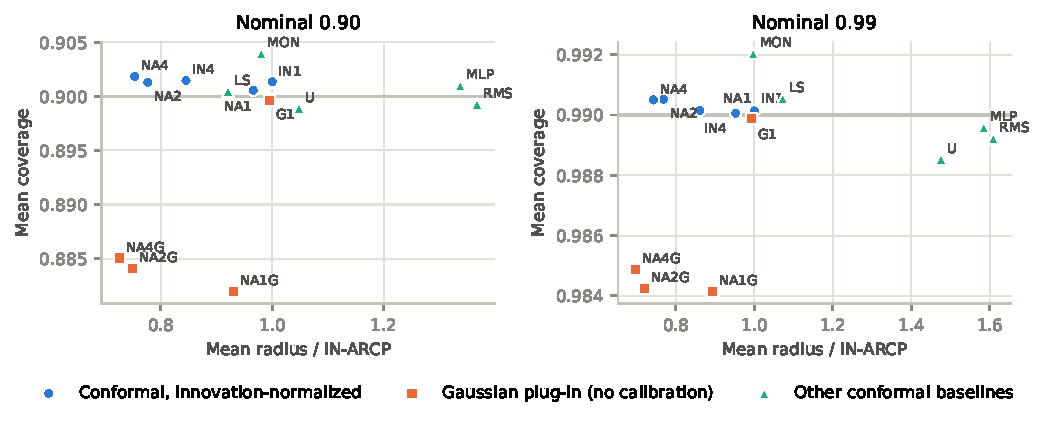
\includegraphics[width=.8\textwidth]{fig_coverage_size.pdf}
\caption{Mean coverage against mean radius (confirmatory, $m=16$). Gaussian plug-ins of the richer noise-aware models are shorter but under-cover; conformal calibration restores nominal coverage. Labels: NA$p$ and IN$p$, noise-aware and innovation-normalized AR($p$) (IN1 is IN-ARCP); G1 and NA$p$G, Gaussian plug-ins; MON, Mondrian; LS, learned scale; U, unnormalized; RMS, raw-RMS; MLP, neural center.}
\end{figure}

\section{Detection study: all levels and methods}\label{sup:detect}
\begin{figure}[h]
\centering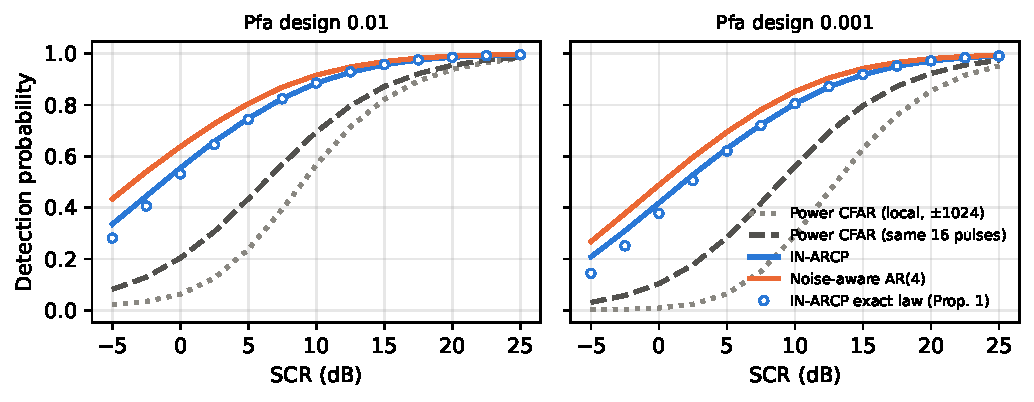
\includegraphics[width=.85\textwidth]{fig_detection.pdf}
\caption{Detection of injected Swerling-1 targets on IPIX at design false-alarm probabilities 0.01 and 0.001.}
\end{figure}
\noindent Pooled detection probability by SCR, measured false-alarm rates, exact-law predictions and SCR gains with 95\% day-cluster intervals (output of \texttt{detection/analyze\_detection.py}):
\VerbatimInput[fontsize=\tiny]{data/detection_summary.txt}

\section{Persistent targets after onset}
Frozen onset study (\texttt{detection/PROTOCOL\_ONSET.md}): per-look detection probability, cumulative detection within $K$ looks, and clean cumulative false-alarm probabilities:
\VerbatimInput[fontsize=\tiny]{data/onset_summary.txt}
\noindent Exploratory: comparison at equal dwell false-alarm probability (0.01), with max and sum-of-squares dwell statistics:
\VerbatimInput[fontsize=\tiny]{data/dwell_summary.txt}
\noindent Exploratory: exact-law prediction of the post-onset decay:
\VerbatimInput[fontsize=\tiny]{data/onset_theory.txt}

\section{Numerical checks of the detection theory}
Monte Carlo checks of Corollary~2, Proposition~2 (closed forms) and Proposition~3 (output of \texttt{detection/theory\_checks.py}):
\VerbatimInput[fontsize=\tiny]{data/theory_checks_output.txt}

\section{Baselines: parametric texture and adaptive conformal inference}
\VerbatimInput[fontsize=\tiny]{data/baselines_summary.txt}


\section{Classical detectors, gradual emergence and ACI contamination (R10)}
Frozen protocol \texttt{r10/PROTOCOL\_R10.md}; stated expectations and verdicts in \texttt{r10/RESULTS\_R10.md}. Output of \texttt{r10/analyze\_r10.py}:
\VerbatimInput[fontsize=\tiny]{data/r10_summary.txt}
\noindent Exact-law prediction of IN-ARCP's per-look detection probability under gradual emergence (endpoint R2):
\VerbatimInput[fontsize=\tiny]{data/theory_ramps.txt}


\section{Order-statistic normalization and real interference (R11)}
Frozen protocol \texttt{r11/PROTOCOL\_R11.md}; expectations and verdicts in \texttt{r11/RESULTS\_R11.md} (2 of 11 met). Monte Carlo check of Corollary~3 (\texttt{r11/theory\_os.py}):
\VerbatimInput[fontsize=\tiny]{data/theory_os_output.txt}
\noindent Output of \texttt{r11/analyze\_r11.py} (Part O: IPIX; Part J: 77~GHz with real interference; N: no zeroing, Z: fast-time zeroing; strata: number of interference-hit chirps among the 16 history chirps):
\VerbatimInput[fontsize=\tiny]{data/r11_summary.txt}

\section{Audit of existing outcomes: conditional false-alarm rates, dependence, leave-one-day-out, fit diagnostics}
Output of \texttt{r10/audit\_existing.py} (descriptive and sensitivity analyses requested in review; no new runs):
\VerbatimInput[fontsize=\tiny]{data/audit_existing.txt}
\noindent Exploratory: sensitivity of NA-AR(4) to optimizer convergence (restart from the capped solution for up to 4,500 further Nelder--Mead iterations; \texttt{r10/explore\_na4\_convergence.py}):
\VerbatimInput[fontsize=\tiny]{data/na4_convergence.txt}

% R12 proofs of the whitened-innovation laws. Numerical checks: research/r7c/r12/verify_laws_output.txt.
\section{Proofs of the whitened-innovation laws}\label{sup:r12proofs}
Throughout, $z\sim\mathcal{CN}(0,I)$ denotes whitened clutter innovations (unit variance after dividing by $\sigma_e$), $g\sim\mathcal{CN}(0,1)$ the Swerling-1 amplitude, and $u$ the whitened target signature, so that the whitened episode is $z+gu\sim\mathcal{CN}(0,I+uu^{\mathsf H})$. $E$, $E_\pm$ are standard exponentials and $\Gamma_k$ a Gamma$(k,1)$ variable, all independent.

\subsection{Proposition (post-onset rank-one law)}
Write the detection event as $F>0$ with $F=x^{\mathsf H}Mx$, $x=z+gu$ and $M=\operatorname{diag}(-\beta I_m,1)$, $\beta=q^2/m$. As in Appendix~\ref{M-app:law} of the paper, $F\overset{d}{=}\sum_k\lambda_kE_k$ with $\lambda_k$ the eigenvalues of $C^{1/2}MC^{1/2}$, $C=I+uu^{\mathsf H}$, which are those of $MC=M+(Mu)u^{\mathsf H}$. For a rank-one update of a diagonal matrix,
\[
\det(\lambda I-M-Muu^{\mathsf H})=\det(\lambda I-M)\Big(1-\sum_i\frac{M_{ii}|u_i|^2}{\lambda-M_{ii}}\Big)=(\lambda-1)(\lambda+\beta)^m\Big(1-\frac{\mathcal E_0}{\lambda-1}+\frac{\beta \mathcal E_H}{\lambda+\beta}\Big),
\]
with $\mathcal E_0=|u_Y|^2$ and $\mathcal E_H=\|u_H\|^2$. Hence $-\beta$ is an eigenvalue of multiplicity $m-1$ and the other two solve $(\lambda-1)(\lambda+\beta)-\mathcal E_0(\lambda+\beta)+\beta\mathcal E_H(\lambda-1)=0$, which is the quadratic of the proposition. Their product is $-\beta(1+\mathcal E_0+\mathcal E_H)<0$, so $\lambda_+>0>\lambda_-$. Then
\[
\PP\{F>0\}=\PP\{\lambda_+E_+>|\lambda_-|E_-+\beta\Gamma_{m-1}\}=\mathbb E\,e^{-(|\lambda_-|E_-+\beta\Gamma_{m-1})/\lambda_+}=\frac{\lambda_+}{\lambda_++|\lambda_-|}\Big(1+\frac{\beta}{\lambda_+}\Big)^{-(m-1)}.
\]
For $\mathcal E_H=0$ the roots are $1+\mathcal E_0$ and $-\beta$, and the expression reduces to $(1+\beta/(1+\mathcal E_0))^{-m}$. The signature of a persistent target follows from the whitened amplitudes in \eqref{M-eq:whitenedscr}: the onset innovation carries $S_w$, every later one $S_w|d|^2$.

\subsection{Corollary (visibility horizon)}
With $\mathcal E_0=S_wD$ and $\mathcal E_H=S_w(1+(\ell-1)D)$, $D=|d(\omega)|^2$, the linear coefficient is $B=1-\beta+S_w\chi$, $\chi=D-\beta\{1+(\ell-1)D\}$, and $\lambda_\pm=\{B\pm(B^2+4\beta(1+\mathcal E_0+\mathcal E_H))^{1/2}\}/2$ with $1+\mathcal E_0+\mathcal E_H=O(S_w)$. If $\chi>0$, then $\lambda_+\sim S_w\chi\to\infty$ while $\lambda_-$ stays bounded, so $P_{\rm d}\to1$. If $\chi<0$, then $\lambda_+\to\beta(1+\ell D)/|\chi|$ stays bounded while $\lambda_-\sim S_w\chi\to-\infty$, so $\lambda_+/(\lambda_+-\lambda_-)\to0$ and $P_{\rm d}\to0$. The sign change $\chi=0$ is $\ell=1+1/\beta-1/D$.

\subsection{Order-statistic scale}
Conditional on $G=|g|^2$, the history powers $|z_j+gu_j|^2$ are independent, exponential for clean innovations and non-central (with $2|z_j+gu_j|^2\sim\chi^2_2(2G|u_j|^2)$) for contaminated ones. The distribution function of their $k$-th smallest value $X_{(k)}$ is the Poisson-binomial probability that at least $k$ are below $x$, and $P_{\rm d}=\mathbb E_G\int\PP\{|z_Y+gu_Y|^2>q^2x\mid G\}\,dF_{X_{(k)}\mid G}(x)$. The code evaluates this by midpoint quadrature in the distribution function of $G$ and a dynamic program for the Poisson-binomial law. If $\ell\le m-k$ contaminated powers diverge, $X_{(k)}$ is the $k$-th smallest of the $m-\ell$ clean ones, which is independent of $z_Y$, and the OS-CFAR law with $m-\ell$ cells gives \eqref{M-eq:osstrong}. If $\ell>m-k$, $X_{(k)}$ diverges with the target while $|z_Y+gu_Y|^2/X_{(k)}$ tends to a constant below any practical threshold, as in Proposition~3.

\subsection{Dwell integration}
Under $H_0$ the event is $\Gamma_K>\tau\Gamma_m$, and conditioning on $\Gamma_m$ with the Poisson form of the Gamma tail gives $\sum_{i<K}\mathbb E[e^{-\tau\Gamma_m}(\tau\Gamma_m)^i/i!]=\sum_{i<K}\binom{m+i-1}{i}\tau^i(1+\tau)^{-(m+i)}$. With a Swerling-1 target the dwell form has one eigenvalue $\delta=1+\mathcal E_D$ and $K-1$ unit ones. For $v>0$,
\[
\PP\{\delta E+\Gamma_{K-1}>v\}=\PP\{\Gamma_{K-1}>v\}+e^{-v/\delta}(1-1/\delta)^{-(K-1)}\PP\{\Gamma_{K-1}\le v(1-1/\delta)\}.
\]
Averaging over $v=\tau\Gamma_m$ uses $\mathbb E e^{-s\Gamma_m}=(1+s)^{-m}$ and $\mathbb E[e^{-s\Gamma_m}\PP\{\Gamma_{K-1}>\tau'\Gamma_m\mid\Gamma_m\}]=\sum_{i\le K-2}\binom{m+i-1}{i}\tau'^{\,i}(1+s+\tau')^{-(m+i)}$ with $s+\tau'=\tau$, which gives \eqref{M-eq:dwellpd}.

\subsection{Self-normalized whitened Doppler}
With a known on-grid Doppler, the whitened dwell vector splits into its DFT coefficient on the target bin, $|\,\cdot\,|^2\sim(1+NS_w|d|^2)E$, and the orthogonal remainder $\Gamma_{N-1}$. The statistic $X/(X+\Gamma_{N-1})$ exceeds $t$ iff $X(1-t)>t\Gamma_{N-1}$, which has probability $\{1+t/((1-t)(1+NS_w|d|^2))\}^{-(N-1)}$; at $S_w=0$ this is $(1-t)^{N-1}$. For the maximum over the $N$ bins, let $I_j$ be independent exponentials with means $\mu_j$ and $J$ a set of bins with $|J|t<1$. Substituting $x_j=tT+y_j$ for $j\in J$, where $T=\sum_iI_i$, the map has Jacobian $1/(1-|J|t)$ and turns the exponent into a sum of independent exponentials, so
\[
\PP\{I_j>tT\ \forall j\in J\}=\frac{1}{1-|J|t}\prod_{i=1}^N\frac{1}{1+\theta_J\mu_i},\qquad\theta_J=\frac{t\sum_{j\in J}\mu_j^{-1}}{1-|J|t},
\]
and zero if $|J|t\ge1$. With all $\mu_i=1$ this is $(1-|J|t)^{N-1}$, and inclusion–exclusion gives Fisher's law $\sum_r(-1)^{r-1}\binom Nr(1-rt)^{N-1}$ (R.~A. Fisher, Proc.\ R.\ Soc.\ Lond.\ A 125, 1929). With one bin of mean $1+NS_w|d|^2$, inclusion–exclusion over sets that do or do not contain it gives $P_{\rm d}$ (\texttt{laws.pd\_snd\_max}).

\subsection{Theorem (certified integration)}
\emph{Domination.} Let $\mathcal J_H$ and $\mathcal J_D$ be the corrupted history and dwell innovations. The $k_H$-th smallest of the history powers is a nondecreasing function of each power, so over all values of the corrupted entries it is smallest when they are zero; hence $s_{k_H}^2\ge\underline s^2$, the value computed with those entries set to zero. Every uncorrupted dwell term is a clean power divided by $s_{k_H}^2\ge\underline s^2$, and every clipped term is at most $\kappa$. Therefore $T\le W$ for all interference values. For binary integration, an uncorrupted exceedance of the actual statistic is an exceedance at $\underline s^2$, and a corrupted term counts at most one. Adding elements to $\mathcal J$ can only lower $\underline s^2$ and replace terms by their maximum, so $W$ is nondecreasing in $\mathcal J$.
\emph{Calibration.} Let the test hit set $\mathcal J$ be independent of the clutter and let $\tilde{\mathcal J}\sim\mathcal D$ with $\mathcal J\subseteq\tilde{\mathcal J}$ (a coupling that exists when $\mathcal D$ dominates the law of $\mathcal J$ in the inclusion order, by Strassen's theorem; a bound on the hit rate alone does not suffice). Then $T\le W(X,\mathcal J)\le W(X,\tilde{\mathcal J})$. The pairs $(X_i,\mathcal J_i)$ and $(X,\tilde{\mathcal J})$ are exchangeable, so the split-conformal rank argument gives $\PP\{W(X,\tilde{\mathcal J})>\widehat q\}\le\alpha$. No property of the interference values is used, so the bound holds for adversarial amplitudes chosen after seeing the clutter, as long as the hit positions are independent of the clutter.
\emph{Trimmed sums.} If a corrupted dwell term can take any value, the trimmed sum over the $K-t$ smallest terms is unbounded once more than $t$ dwell terms are corrupted, which a Bernoulli hit model allows with positive probability. The conformal quantile of the worst case is then infinite whenever that probability exceeds $\alpha$.

\subsection{Conformal calibration size and loss}
For continuous i.i.d. scores the $k_\alpha$-th order statistic of $n$ calibration scores, mapped through the score distribution function, is Beta$(k_\alpha,n+1-k_\alpha)$; the conditional false-alarm probability is one minus it, hence Beta$(n+1-k_\alpha,k_\alpha)$. Because $k_\alpha$ is a ceiling, $\PP\{P_{\rm fa}>2\alpha\}$ is not monotone in $n$; an exhaustive scan (\texttt{laws.n\_required}) gives the smallest $n$ and the $n$ beyond which the condition always holds. With ties the rank argument still gives $\PP\{T>\widehat q\}\le\alpha$, but the Beta law no longer applies. For $P_{\rm d}=P_{\rm fa}^{\gamma}$, $\mathbb EU^\gamma=B(n+1-k_\alpha+\gamma,k_\alpha)/B(n+1-k_\alpha,k_\alpha)$, with $B$ the Beta function.


\section{R12: Monte Carlo checks, full results and verdicts}\label{sup:r12}
Frozen protocol \texttt{r12/PROTOCOL\_R12.md} (sha256 a32706e7\ldots); expectations and verdicts in \texttt{r12/RESULTS\_R12.md} (12 of 18 met). Monte Carlo checks of most closed forms in Section~\ref{M-sec:laws} (\texttt{r12/verify\_laws.py}, 400,000 replications); the guarded law and an independent re-check are in Section~\ref{sup:indep}. The V7 rows marked ``law assumes Gaussian'' test the Kraut--Scharf law with compound-Gaussian secondary data, where it fails 2.8--3.4-fold; they are excluded from the $|z|$ summary because that law does not claim to hold there. The summary's 65 checks are the rows with a $z$-score, less every row with a bracketed label (the two rows just named, and the four rows of the asymptotic fixed-point law, whose $|z|<1.6$); the V8 Beta-law rows and the V9 certificate rows report agreement or violation rates, not $z$-scores. The printed maximum 2.91 is rounded from 2.9125; each of the 65 lies within 3 standard errors. The calibration sizes printed under V8 came from a faulty search and are superseded by \texttt{r12/calibration\_size.txt} (149, 1,497 and 14,978; every $n$ beyond 313, 3,146 and 31,477):
\VerbatimInput[fontsize=\tiny]{data/verify_laws_output.txt}
\noindent IPIX parts L (low false-alarm calibration), A (dwell detection with ANMF baselines), T (real target) and I (injected pulsed interference), with 95\% day-cluster intervals (\texttt{r12/analyze\_r12.py}):
\VerbatimInput[fontsize=\tiny]{data/r12_summary.txt}
\noindent 77~GHz data with real interference (\texttt{r12/analyze\_r12\_jku.py}); N: no fast-time mitigation, Z: zeroing, ZAR: zeroing with AR(8) gap reconstruction; strata: number of hit chirps in the 24-chirp segment (0, 1--2, 3--5, $\ge6$):
\VerbatimInput[fontsize=\tiny]{data/r12_jku_summary.txt}

% Generated by analysis_provenance/make_supp_sections.py from the saved outcomes. Do not edit.
\section{Guarded scale, clip level, certified trimming, pulse blanking and bursts (R14)}\label{sup:r14}
Frozen protocol \texttt{r14/PROTOCOL\_R14.md} (sha256 9f771091\ldots), written after a synthetic dry run and before any IPIX outcome; expectations and verdicts in \texttt{r14/RESULTS\_R14.md} (12 of 15 met). The settings are those of the final IPIX study, except for dense calibration: non-overlapping 24-pulse segments, about 14,600 per unit, so that $\alpha=10^{-3}$ is resolved. The study tested five changes:
\begin{itemize}
\item a guard of $\Delta\in\{0,8,16\}$ pulses between the scale window and the tested pulse;
\item clip levels $\kappa\in\{4,6,9,12,18\}$;
\item a certified trimmed sum, which discards the largest dwell terms; the number discarded is the smallest for which more corrupted dwell innovations than discarded terms have probability at most $\alpha/5$ under the hit model (4 of eight at a 2\% and 5 at a 5\% hit rate at $\alpha=10^{-2}$; no such number exists for bursts);
\item pulse blanking of isolated spikes, calibrated with masks drawn from the hit model and passed through the same rule (mask-matched calibration);
\item bursts of eight consecutive pulses at the same mean hit rate.
\end{itemize}
The certified thresholds use the worst case of Theorem~\ref{M-thm:cert} with hits drawn either from the independent-hit model or from the burst model. The guard leaves the false-alarm law unchanged; the measured $P_{\rm fa}/\alpha$ with $\Delta=8$ is 1.03 at $10^{-2}$ and 1.03 at $10^{-3}$. The real IPIX target stays undetected with every guard (exceedance 0.0005 at $10^{-3}$ with $\Delta=8$), because it is present in every history.

\emph{Unmet expectations of R14.}
\begin{itemize}
\item \textbf{Onset cost (G3).} The guard was expected to cost at most 0.5~dB at onset. It costs 0.9~dB with $\Delta=8$ and 1.2~dB with $\Delta=16$, because the scale is older.
\item \textbf{Certification at $10^{-3}$ (K2).} The certificate at the clip level chosen by the saturation rule was expected to reach $P_{\rm d}=0.5$ below 25~dB in all four interference conditions at $10^{-3}$. With 5\% hits the certificate is vacuous at $10^{-3}$ for every clip level.
\item \textbf{Cost of trimming (T2).} Trimming was expected to cost more than clipping at both hit rates. At 5\% it costs +5.1~dB against +5.9~dB for clipping ($\kappa=6$).
\end{itemize}
The SCR for $P_{\rm d}=0.5$ is fragile under 5\% hits, because the certified detection curve is nearly flat there, so the main text reports $P_{\rm d}$ at 10~dB.

\noindent Output of \texttt{r14/analyze\_r14.py}. Columns of the interference table: condition, $\alpha$, statistic, pooled $P_{\rm fa}/\alpha$ [upper day-cluster bound], SCR for $P_{\rm d}=0.5$, its cost against clean clipping ($\kappa=6$), and $P_{\rm d}$ at 10 and 25~dB.
\VerbatimInput[fontsize=\tiny]{data/r14_summary.txt}

\section{Independent re-check of the main laws and of Theorem~\ref{M-thm:cert}}\label{sup:indep}
\texttt{r14/theory\_check\_independent.py} re-derives the main closed forms of Section~\ref{M-sec:laws} and Theorem~\ref{M-thm:cert} by Monte Carlo on a GPU (the remaining laws are checked by the study scripts, Section~\ref{sup:r12}). It was written from scratch and does not import the code that implements the laws. It checks:
\begin{itemize}
\item Proposition~\ref{M-prop:law}, including repeated eigenvalues and a singular $Q$;
\item Proposition~\ref{M-prop:rank1};
\item the horizon of Corollary~\ref{M-cor:horizon};
\item the strong-target OS law \eqref{M-eq:osstrong}, the integration laws and the known-bin P-ANMF law;
\item the Beta law (by Monte Carlo) and the calibration sizes (by exact computation);
\item Theorem~\ref{M-thm:cert} under strong, matched and cancelling interference.
\end{itemize}
It also includes a misspecified case: bursts against a certificate calibrated on independent hits, which violates the dominance condition. There the clipped certificate exceeds $\alpha$, as the theorem's condition implies it may.
\VerbatimInput[fontsize=\tiny]{data/theory_check_independent_output.txt}
\noindent The guarded post-onset law (Proposition~\ref{M-prop:rank1} with $\ell$ replaced by $\ell-\Delta$) is checked separately by \texttt{r14/theory\_check\_guard.py}, also written from scratch. With $\Delta=8$ the decay is that of $\Delta=0$ delayed by eight looks:
\VerbatimInput[fontsize=\tiny]{data/theory_check_guard.txt}
\noindent The line for $n=23{,}000$ checks the formula only. The low-false-alarm calibration sets have 17,200--23,100 episodes per unit, for which the same formula gives $\PP\{P_{\rm fa}>2\alpha\}=0.02$--0.09 (Section~\ref{M-sec:calib}).

\section{The real IPIX target: detection versus dwell length}\label{sup:target}
\begin{table}[h]
\centering\small
\caption{Real IPIX target (primary cell, test thirds, 56 units): mean $P_{\rm d}$ at design $P_{\rm fa}=10^{-3}$ versus dwell $N$. In parentheses: measured clutter $P_{\rm fa}$ ($\times10^{-3}$). P-ANMF with Fisher's $g$ uses the analytic threshold.}
\label{tab:target}
\begin{tabular}{rcccc}
\toprule
 & \multicolumn{2}{c}{P-ANMF} & Range CA & ANMF\\
\cmidrule(lr){2-3}
$N$ & conformal & Fisher's $g$ & integration & Tyler\\
\midrule
8 & 0.22 (1.1) & 0.37 (13) & 0.003 & 0.13\\
16 & 0.22 (1.3) & 0.45 (32) & 0.003 & 0.18\\
32 & 0.22 (1.3) & 0.56 (69) & 0.004 & --\\
64 & 0.30 (1.3) & 0.67 (121) & 0.004 & --\\
128 & 0.37 (1.2) & 0.75 (178) & 0.004 & --\\
256 & 0.40 (1.5) & 0.79 (235) & 0.004 & --\\
512 & 0.37 (2.0) & 0.83 (299) & 0.005 & --\\
1024 & 0.41 (2.6) & 0.87 (404) & 0.007 & --\\
\bottomrule
\end{tabular}

\end{table}
Calibration of the self-normalized detector degrades for longer, overlapping windows. Its analytic Fisher's $g$ threshold fails already at $N=8$, consistent with imperfect whitening by an AR(4) model fitted on neighboring cells. The value of P-ANMF here is a calibrated short-dwell threshold, not sensitivity.

\section{77~GHz data: receivers, range bins and thermal noise}\label{sup:jkusel}
Range bins 8--247 of receivers 0, 5, 10 and 15 of both stations are used. As the CNR rises from noise-dominated cells to 10--20~dB, the measured gain of IN-ARCP over local power detection rises from $-1.45$~dB to $3.11$~dB, following the sign of Proposition~\ref{M-prop:gain}.

\section{Further detector notes}\label{sup:notes}
\begin{itemize}
\item \textbf{Power-detector laws.} At $10^{-3}$ the white-noise laws of the power detectors err in both directions: CA16 runs at 0.56 times design and the OS detector on raw powers at 5.56 times design.
\item \textbf{OS variants after onset.} The OS variants with $k=12$ and with AR(4) innovations collapse at the first look at which the target occupies more than $m-k$ history innovations, as \eqref{M-eq:osstrong} states. The pre-specified count was off by one and was corrected after the data were seen (Section~\ref{sup:deviations}).
\item \textbf{Worst case in Theorem~\ref{M-thm:cert}.} The worst case over amplitudes is attained for the clipped dwell terms, which strong interference drives to $\kappa$. It is conservative only through the history scale, whose corrupted entries are set to zero.
\item \textbf{Certified binary integration.} In the final IPIX study (R12, sparse calibration), the detection probability of certified binary integration for a 10~dB target was within 0.03 of that of certified clipping at both hit rates and powers (output in Section~\ref{sup:r12}).
\end{itemize}

% Generated by analysis_provenance/make_supp_sections.py from the saved outcomes. Do not edit.
\section{Second sea-clutter radar: NetRAD (R15)}\label{sup:r15}
Frozen protocol \texttt{r15/PROTOCOL\_R15.md} (sha256 945c5e51\ldots). It was written before any statistic of the NetRAD samples was computed. Before that point only the following had been read: file sizes, array shapes, and the providers' scripts and log. In addition, two of the providers' own quick-look images were viewed while the dataset was being located. Expectations and verdicts are in \texttt{r15/RESULTS\_R15.md} (12 of 15 met), and deviations in \texttt{r15/DEVIATIONS\_R15.md}. The deviations are a corrected site description (the Atlantic side of the Cape Peninsula, not False Bay) and run mechanics; none changes a method, setting or expectation.

\emph{Data.} Node 3 (monostatic) of the NetRAD system: seven HH and seven VV recordings of 130{,}000 pulses at 1~kHz. The clutter cells are the providers' per-recording range windows (\texttt{NR\_Range\_Selection\_June9.m}). Each cell has its complex mean removed and is scaled to unit power. The cross-polarized recordings were set aside before any data were read. All methods are the frozen R12 and R14 code. The only change is that the ANMF secondary cells are restricted to those two to four cells away, which gives 15--30 vectors (20--35 on IPIX). The AR(1) clamp $|r|\le0.98$ binds in 12 of the 14 recordings.

\emph{Unmet expectations of R15.}
\begin{itemize}
\item \textbf{Calibration at $10^{-4}$ (N1).} At least 12 of 13 conformal ratios were expected within $[0.5,2]$ at $10^{-4}$; 7 were. Outside: Clip-OS1 (0.39), D-IN4 (4.26), NA4 (2.08), P-ANMF (2.33), P-ANMF(bin) (2.52), PAMF-H(w) (2.18). At $10^{-3}$ all 13 are within $[0.5,2]$, and the 12 non-saturating statistics lie within 1.01--1.36 times design.
\item \textbf{Pivotality ranking (N4).} IN-ARCP's quintile spread at $10^{-2}$ was expected to be at most 2 and below CA16's. It is 2.40 against 1.51. In the same analysis on IPIX it is 1.31 against 1.06, so this expectation had no support on IPIX either.
\item \textbf{Flagged pulses (W2).} Non-coherent integration with a clean threshold was expected to exceed $1.5\alpha$ in segments with flagged pulses. It stays at 1.08 times design.
\end{itemize}
Expectation N5 (PAMF-H within 0.5~dB of the best dwell detector) was met, but it is uninformative: every whitened dwell detector reaches $P_{\rm d}=0.5$ at the lowest SCR tested.

\emph{Exploratory (post hoc, after the outcomes and the claim audit).} Two scripts look at where the conformal exceedances at $10^{-4}$ fall: \texttt{r15/explore\_r15\_hotspots.py} and \texttt{r15/explore\_r15\_attribution.py}.
\begin{itemize}
\item \textbf{Integration and PAMF-H.} Most of their excess comes from two VV units (1450 and 1501, assignment 3). Their exceedances fall within one to three seconds of the test third and coincide with flagged pulses, while their calibration thirds contain no flagged pulse. Without these two units the pooled ratios are 1.56 (integration) and 1.33 (PAMF-H).
\item \textbf{P-ANMF statistics.} Their excess comes from one HH unit (1128, assignment 3) with frequent flagged pulses in both thirds. Fewer than half of its exceedances coincide with flagged pulses.
\item \textbf{Unexplained.} The flagged pulses do not explain the excess of the noise-aware score (2.08). Nor do they explain an excess of integration of more than five times design in one unit that has no flagged pulse at all (1508, assignment 2).
\end{itemize}
\textbf{What the flags are is not established.} \texttt{r15/explore\_r15\_flag\_extent.py} counts, in the raw recordings, the range bins above ten times their median:
\begin{itemize}
\item a flagged HH pulse has a median of about 108 such bins, of 1024, and 85--91\% of them lie outside the clutter window;
\item unflagged HH pulses with an elevated window bin have about 80.
\end{itemize}
The flags are therefore the upper tail of a phenomenon that extends over range. They may be wideband interference: the providers remove WiFi pulses in their own processing of the bistatic nodes. They may equally be range-extended HH sea spikes. The main text therefore calls them flagged pulses, not interference.

In the clutter cells, uncertified non-coherent integration runs at 1.05 times design at $10^{-2}$ and 1.20 at $10^{-3}$ over all test segments of the 7 HH recordings, the only ones with at least 0.5\% flagged pulses (VV: at most 0.1\%). Segments without a flagged pulse give 1.04 and 1.17; segments with flagged pulses give at most 1.08 and 1.33, with wide intervals at $10^{-3}$ (Part W below). A certificate whose hit model must cover these frequent, bursty masks is nearly vacuous ($P_{\rm d}=0.04$). Blanking with mask-matched calibration keeps $P_{\rm d}=0.92$ at 0.57 times design.

\noindent Output of \texttt{r15/analyze\_r15.py} (Parts L, A, G, I, K/X/B and W; intervals resample recordings):
\VerbatimInput[fontsize=\tiny]{data/r15_summary.txt}
\noindent Exploratory hotspot analysis (\texttt{r15/explore\_r15\_hotspots.py}):
\VerbatimInput[fontsize=\tiny]{data/r15_hotspots.txt}
\noindent Exploratory attribution (\texttt{r15/explore\_r15\_attribution.py}): flagged-pulse fraction in each unit's calibration and test thirds, the per-unit ratios at $10^{-4}$, and the pooled ratios without the units named above:
\VerbatimInput[fontsize=\tiny]{data/r15_attribution.txt}
\noindent Exploratory range extent of the flagged pulses (\texttt{r15/explore\_r15\_flag\_extent.py}):
\VerbatimInput[fontsize=\tiny]{data/r15_flag_extent.txt}

\section{Real onsets of a walking person at 77~GHz (R17)}\label{sup:r17}
Frozen protocol \texttt{r17/PROTOCOL\_R17.md}, committed and pushed before the data were obtained; verdicts in \texttt{r17/RESULTS\_R17.md}. In the pedestrian run of the 77~GHz data (\texttt{meas\_3\_int\_A\_pedestrian}, interference scenario A) a person walks in front of Station 1. Frames are 200~ms apart, so the person moves through the 15-cm range bins between frames, and each arrival of its return in a bin is a real onset in that bin's frame-to-frame sequence. Because the receivers are real-valued, Station 1 sees the person twice: directly, and bistatically via Station 2's transmission, about 130 bins (19~m) farther in this run. The 74 onsets are those of both returns (38 direct, 36 bistatic) in adjacent bins over 31 frames, so they are not independent arrivals.

\emph{Ground truth.} Station 1's range-Doppler map over all 128 chirps and 16 receivers (fast-time zeroing). A bin is moving in a frame when its largest power over Doppler bins at least two from zero exceeds its median over the 100 frames by 10~dB. An onset is a bin that becomes moving after 16 frames without moving energy; it is the person's when one of the frame's two strongest moving peaks (13~dB) lies within three bins in the onset frame or the next two.

\emph{Detectors.} One chirp per frame (chirps 0, 32, 64, 96; receivers 0, 5, 10, 15: 16 looks), history of 16 frames: IN-ARCP (AR(1) per bin, fitted on clean frame pairs), the power clutter map (CA-CM: power over the mean history power), its OS form (OS-CM: eighth smallest of 16) and range CA-CFAR on the current frame (2 guard and 8 reference bins on each side). Conformal thresholds from null episodes of even bins, false alarms on odd bins. The primary endpoint is detection within three frames of the onset.

\emph{Outcome.} The protocol required onsets in at least eight distinct five-frame blocks; the person was tracked for about six seconds and the onsets fall in seven, so expectation E1 is not met and every result is descriptive. Descriptively, all lie on the side the protocol expected: false-alarm rates at design, IN-ARCP $\ge$ CA-CM $>$ OS-CM $>$ range CA-CFAR, and IN-ARCP's edge over CA-CM confined to the half of the onsets in bins with stronger static returns, as Proposition~\ref{M-prop:gain} predicts for nearly uncorrelated frame-to-frame clutter. \emph{Limitations} (stated as the protocol requires): one walk, tracked for about six seconds, by one person; ground clutter at 77~GHz, not sea clutter; frame-rate rather than pulse-rate slow time; ground truth from the same radar's range-Doppler processing, with no external sensor. Before the expectations were written, a mechanics check ran the whole chain on the interference run without the pedestrian, with a synthetic walker; its output, including the four detectors' detection rates for that walker, is \texttt{r17/MECHANICS\_R17.txt}. The onset rule, the three-frame endpoint and the expectations were set after this check, and the AR(1) coefficient is fitted on the same file as the test.

Output of \texttt{run\_r17\_jku.py}, long lines wrapped (intervals are understated with seven blocks):
\VerbatimInput[fontsize=\tiny]{data/r17_summary.txt}

% Generated by analysis_provenance/make_supp_sections.py. Do not edit.
\section{Closed forms against Monte Carlo: all six panels}\label{sup:theoryfig}
\begin{figure}[h]
\centering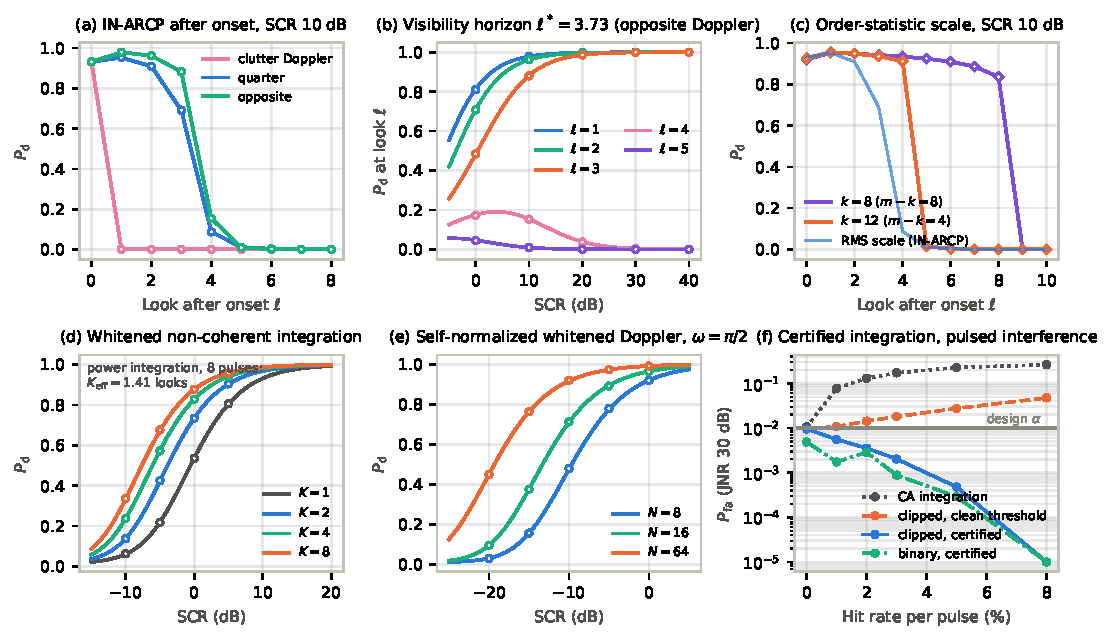
\includegraphics[width=.95\textwidth]{fig_theory_full.pdf}
\caption{Closed forms (lines) against Monte Carlo (markers; $10^5$ episodes per point in (a), (c) and (f), $5\times10^4$ in (b) and (d), $10^4$ to $2.5\times10^4$ in (e)) at the true coefficient, AR(1) compound-Gaussian clutter with $\rho=0.93e^{-0.2\mathrm j}$, lognormal texture, $m=16$, $P_{\rm fa}=0.01$. Panels (a)--(c) and (f) are those of Fig.~\ref{M-fig:theory} of the paper, where (f) appears as its panel (d) and (c) here adds the RMS-scale law for reference. The two panels shown only here are (d), the integration law \eqref{M-eq:dwellpd}, and (e), P-ANMF with unknown Doppler. JNR in (f): interference-to-clutter-plus-noise power ratio.}
\end{figure}

\section{Dwell detection on IPIX}\label{sup:dwell}
\begin{table}[h]
\centering\small
\caption{SCR (dB) for $P_{\rm d}=0.5$ and $0.9$ over an 8-pulse dwell: persistent Swerling-1 target with random Doppler from the first dwell pulse (IPIX, conformal thresholds). $\le-5$: reached at the lowest SCR tested; n.r.: not reached at 25~dB.}
\label{tab:dwellsup}
\begin{tabular}{lccc}
\toprule
 & \multicolumn{2}{c}{$\alpha=0.01$} & $0.001$\\
\cmidrule(lr){2-3}
 Detector & $P_{\rm d}=0.5$ & $0.9$ & $0.5$\\
\midrule
PAMF-H & $\le-5$ & 5.1 & -4.3\\
Integration, AR(4) & $\le-5$ & 7.0 & -1.6\\
Integration, AR(1) & -4.4 & 8.3 & -0.1\\
Clipped, OS scale & -2.3 & 13.0 & n.r.\\
Binary, OS scale & -1.2 & 14.5 & n.r.\\
ANMF-SCM & -0.2 & 20.3 & 9.5\\
ANMF-Tyler & 0.4 & 20.3 & 9.8\\
P-ANMF & 0.2 & n.r. & n.r.\\
IN-ARCP, first look & -1.2 & 11.0 & 1.9\\
Power OS, first look & 9.4 & 19.5 & 14.3\\
\bottomrule
\end{tabular}

\end{table}


\section{77~GHz radar: full results}
\begin{figure}[h]
\centering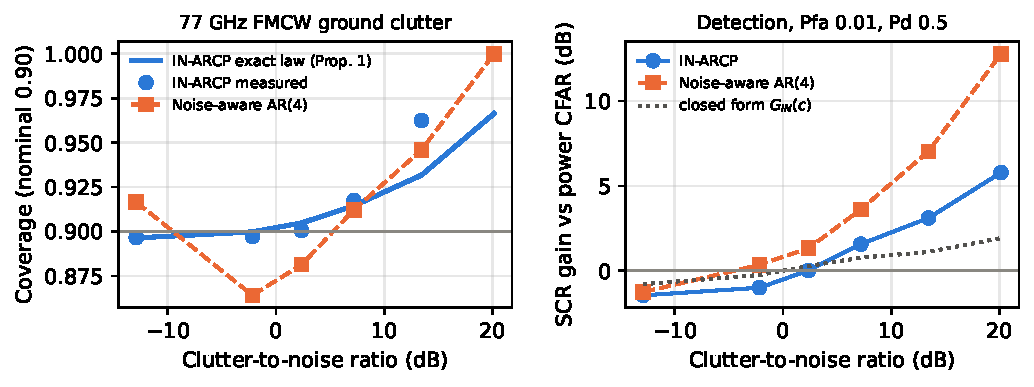
\includegraphics[width=.85\textwidth]{fig_jku.pdf}
\caption{77~GHz FMCW ground clutter: coverage by CNR class with the exact law, and SCR gain over the local power detector.}
\end{figure}
\VerbatimInput[fontsize=\tiny]{data/jku_summary.txt}
\end{document}
